\documentclass[tikz,border=10pt]{standalone}
\usepackage{helvet}
\renewcommand{\familydefault}{\sfdefault}
\usetikzlibrary{arrows.meta, backgrounds, calc, fit, positioning, shapes.geometric}

\colorlet{linecolor}{black}
\colorlet{textmuted}{black!65}
\colorlet{setupfill}{black!10}
\colorlet{artifactfill}{black!6}
\colorlet{decisionfill}{black!14}
\colorlet{branchfill}{black!8}
\colorlet{panelstroke}{black!25}

\tikzset{
  box/.style={
    draw=linecolor,
    thick,
    rounded corners=8pt,
    minimum width=6.4cm,
    minimum height=10.5mm,
    align=center,
    fill=white,
    font=\small
  },
  setup/.style={box, fill=setupfill},
  process/.style={box, fill=white},
  artifact/.style={box, fill=artifactfill},
  decision/.style={
    diamond,
    draw=linecolor,
    thick,
    aspect=2.1,
    align=center,
    fill=decisionfill,
    inner sep=1.2pt,
    minimum width=4.4cm,
    font=\small
  },
  discard/.style={box, fill=branchfill, minimum width=4.9cm},
  keep/.style={box, fill=branchfill, minimum width=4.9cm},
  arr/.style={-{Latex[length=3.0mm,width=2.0mm]}, thick, draw=linecolor},
  note/.style={font=\footnotesize, text=textmuted}
}

\begin{document}
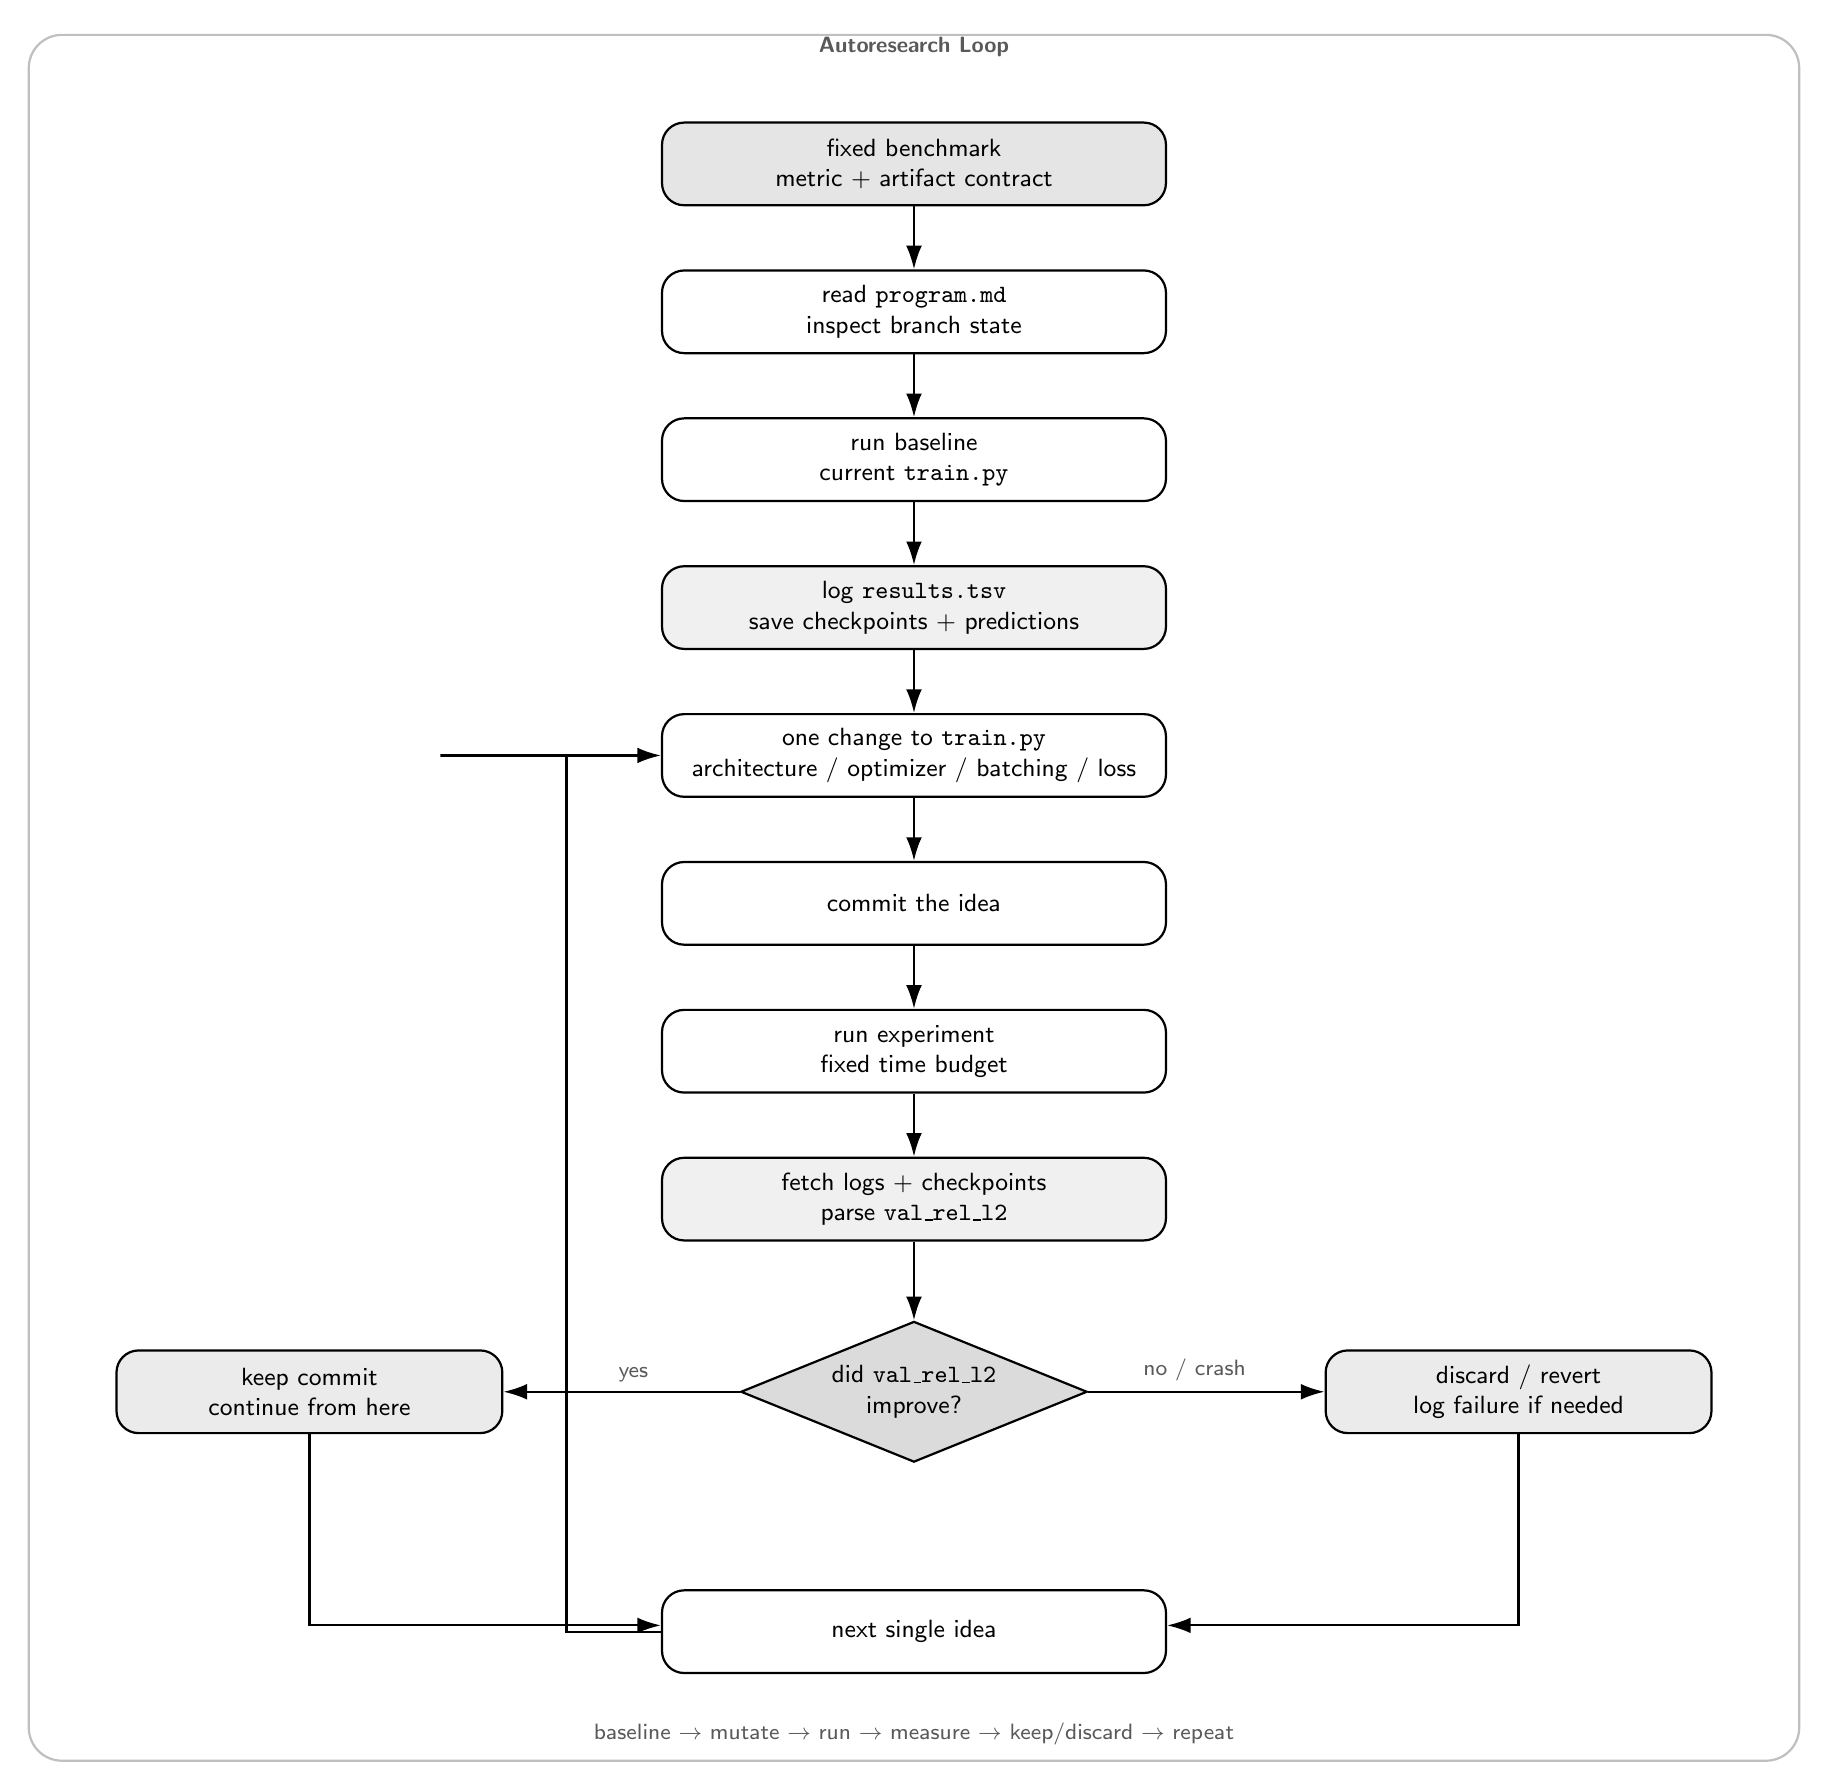
\begin{tikzpicture}[node distance=8mm and 28mm]

\node[setup] (benchmark) {fixed benchmark\\metric + artifact contract};
\node[process, below=of benchmark] (read) {read \texttt{program.md}\\inspect branch state};
\node[process, below=of read] (baseline) {run baseline\\current \texttt{train.py}};
\node[artifact, below=of baseline] (logbase) {log \texttt{results.tsv}\\save checkpoints + predictions};
\node[process, below=of logbase] (mutate) {one change to \texttt{train.py}\\architecture / optimizer / batching / loss};
\node[process, below=of mutate] (commit) {commit the idea};
\node[process, below=of commit] (run) {run experiment\\fixed time budget};
\node[artifact, below=of run] (fetch) {fetch logs + checkpoints\\parse \texttt{val\_rel\_l2}};
\node[decision, below=10mm of fetch] (decision) {did \texttt{val\_rel\_l2}\\improve?};

\node[keep, left=30mm of decision] (keep) {keep commit\\continue from here};
\node[discard, right=30mm of decision] (discard) {discard / revert\\log failure if needed};
\node[process, below=16mm of decision] (next) {next single idea};
\coordinate (loopleft) at ($(mutate.west)+(-28mm,0)$);

\draw[arr] (benchmark) -- (read);
\draw[arr] (read) -- (baseline);
\draw[arr] (baseline) -- (logbase);
\draw[arr] (logbase) -- (mutate);
\draw[arr] (mutate) -- (commit);
\draw[arr] (commit) -- (run);
\draw[arr] (run) -- (fetch);
\draw[arr] (fetch) -- (decision);

\draw[arr] (decision.west) -- node[above, note, pos=0.45] {yes} (keep.east);
\draw[arr] (decision.east) -- node[above, note, pos=0.45] {no / crash} (discard.west);

\draw[arr] (keep.south) |- ($(next.west)+(0,0.8mm)$);
\draw[arr] (discard.south) |- ($(next.east)+(0,0.8mm)$);
\draw[arr] (next.west) -- ++(-12mm,0) |- (loopleft) |- (mutate.west);

\begin{scope}[on background layer]
  \node[
    draw=panelstroke,
    rounded corners=12pt,
    line width=0.8pt,
    fill=white,
    fit=(benchmark)(read)(baseline)(logbase)(mutate)(commit)(run)(fetch)(decision)(keep)(discard)(next),
    inner sep=11mm
  ] {};
\end{scope}

\node[note, above=7mm of benchmark] {\textbf{Autoresearch Loop}};
\node[note, below=5mm of next] {baseline $\rightarrow$ mutate $\rightarrow$ run $\rightarrow$ measure $\rightarrow$ keep/discard $\rightarrow$ repeat};

\end{tikzpicture}
\end{document}
